\documentclass[11pt]{article}
\usepackage[utf8]{inputenc}
\usepackage[margin=5cm]{geometry}
\usepackage{amsmath}
\usepackage{amsthm}
\usepackage{amssymb}
\usepackage{lipsum}
\linespread{1.2}
\usepackage{titlesec}
\usepackage{caption}
\usepackage{tikz}
\usepackage{tkz-euclide}
\usetikzlibrary{angles, quotes, arrows}
\usetkzobj{all}

\titleformat*{\section}{\large\bfseries}

\title{Proof: All Angles are Right Angles}
\author{Gabriel Kammer \hspace{.2cm} Avery Nortonsmith}
\date{January 2020}

\begin{document}

\maketitle

\vspace{1cm}

\begin{center}
    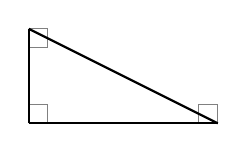
\begin{tikzpicture}[scale=1.2]
        \coordinate (A) at  (0, 0);
        \coordinate (B) at  (2, 0);
        \coordinate (C) at  (0, 1);
        \coordinate (D) at  (2, 1);

        \tkzMarkRightAngle[size=.2,color=gray](B,A,C);
        \tkzMarkRightAngle[size=.2,color=gray](A,B,D);
        \tkzMarkRightAngle[size=.2,color=gray](A,C,D);

        \draw[-, thick] (A) -- (B);
        \draw[-, thick] (A) -- (C);
        \draw[-, thick] (B) -- (C);
    \end{tikzpicture}
\end{center}

\vspace{1cm}

\section{Background}

Last semester my friend Gabe show me a ``proof'' of a stunning result: that all angles are right angles. In the past few months I've had lots of fun showing this proof to others, and watching them move through the stages of bewilderment, denial, and finally acceptance. Like all great mathematical proofs, it is graphical in nature - math notation alone is not powerful enough to capture its subtleties. In this paper, I carefully reproduce the key components of Gabe's original proof, in the hope that it will enlighten others just as it has enlightened me.

\vspace{.2cm}

\hfill \emph{- Avery Nortonsmith}

\newpage

\section{Proof}

We construct the diagram for our proof using the following steps. \emph{Note that all points, line segments, and angles in the figures below occur in the same plane. }

% ----------------------------------------------------------------------------

\subsection{Step 1}

\vspace{.5cm}

\begin{figure}[ht]
    \centering
    \begin{tikzpicture}[scale=1.7]
        \path (0,1) -- (5.5,0);
        \coordinate (A) at  (0, 0);
        \coordinate (B) at  (5, 0);
        \coordinate (C) at  (0, 1);
        
        \tkzMarkRightAngle[size=.2,color=gray](C,A,B);
        
        \filldraw [] (A) circle (1pt) node[below left]{$a$};
        \filldraw [] (B) circle (1pt) node[below right]{$b$};
        \filldraw [] (C) circle (1pt) node[above left]{$c$};
        
        \draw[-, thick] (A) -- (B);
        \draw[-, thick] (A) -- (C);
    \end{tikzpicture}
\end{figure}

\vspace{.5cm}

Start by drawing a horizontal line segment $\overline{ab}$, along with a shorter, vertical segment $\overline{ac}$ such that $\overline{ac} \perp \overline{ab}$.

\vspace{.5cm}

% ----------------------------------------------------------------------------

\subsection{Step 2}

\vspace{.5cm}

\begin{figure}[ht]
    \centering
    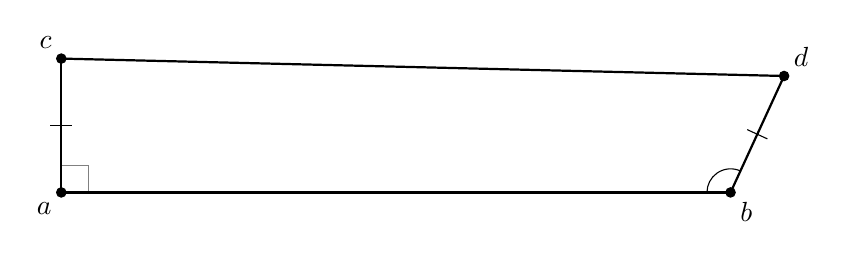
\begin{tikzpicture}[scale=1.7]
        \path (0,1) -- (5.5,0);
        \coordinate (A) at  (0, 0);
        \coordinate (B) at  (5, 0);
        \coordinate (C) at  (0, 1);
        \coordinate (D) at  (5.4, .87);
        
        \tkzMarkRightAngle[size=.2,color=gray](C,A,B);
        
        \draw [-] pic [draw=black, angle radius=3mm, above left] {angle = D--B--A};
        
        \filldraw [] (A) circle (1pt) node[below left]{$a$};
        \filldraw [] (B) circle (1pt) node[below right]{$b$};
        \filldraw [] (C) circle (1pt) node[above left]{$c$};
        \filldraw [] (D) circle (1pt) node[above right]{$d$};
        
        \tkzMarkSegment[mark=|](A, C)
        \tkzMarkSegment[mark=|](B, D)
        
        \draw[-, thick] (A) -- (B);
        \draw[-, thick] (A) -- (C);
        \draw[-, thick] (B) -- (D);
        \draw[-, thick] (C) -- (D);
    \end{tikzpicture}
\end{figure}

\vspace{.5cm}

Next, add segment $\overline{bd}$ with the same length as $\overline{ac}$ such that $\overline{bd}$ forms an obtuse angle $\angle abd$ with $\overline{ab}$. Then, draw a line between $c$ and $d$. Segment $\overline{cd}$ is slightly slanted with respect to $\overline{ab}$, since $\angle abd$ is obtuse.

\newpage

% ----------------------------------------------------------------------------

\subsection{Step 3}

\vspace{.5cm}

\begin{figure}[ht]
    \centering
    \begin{tikzpicture}[scale=1.7]
        \path (0,1) -- (5.5,-2);
        \coordinate (A) at  (0, 0);
        \coordinate (B) at  (5, 0);
        \coordinate (C) at  (0, 1);
        \coordinate (D) at  (5.4, .87);
        \coordinate (E) at  (2.5, 0);
        \coordinate (F) at  (2.62, .93);
        \coordinate (G) at  (2.5, -2);

        \tkzMarkRightAngle[size=.2,color=gray](C,A,B);
        \tkzMarkRightAngle[size=.2,color=gray](C,F,G);
        \tkzMarkRightAngle[size=.2,color=gray](D,F,G);
        \tkzMarkRightAngle[size=.2,color=gray](A,E,G);
        \tkzMarkRightAngle[size=.2,color=gray](B,E,G);

        \draw [-] pic [draw=black, angle radius=3mm] {angle = D--B--A};

        \filldraw [] (A) circle (1pt) node[below left]{$a$};
        \filldraw [] (B) circle (1pt) node[below right]{$b$};
        \filldraw [] (C) circle (1pt) node[above left]{$c$};
        \filldraw [] (D) circle (1pt) node[above right]{$d$};
        \filldraw [] (E) circle (1pt) node[above left]{$e$};
        \filldraw [] (F) circle (1pt) node[above]{$f$};
        \filldraw [] (G) circle (1pt) node[below]{$g$};

        \tkzMarkSegment[mark=|](A, E)
        \tkzMarkSegment[mark=|](B, E)

        \tkzMarkSegment[mark=||](C, F)
        \tkzMarkSegment[mark=||](D, F)

        \draw[-, thick] (A) -- (B);
        \draw[-, thick] (A) -- (C);
        \draw[-, thick] (B) -- (D);
        \draw[-, thick] (C) -- (D);
        \draw[-, thick] (E) -- (G);
        \draw[-, thick] (F) -- (G);
    \end{tikzpicture}
\end{figure}

\vspace{.5cm}

Let points $e$ and $f$ be the midpoints of $\overline{ab}$ and $\overline{cd}$, respectively. Draw the perpendicular bisectors $\overline{eg}$ and $\overline{fg}$ of $\overline{ab}$ and $\overline{cd}$, respectively, where point $g$ is the intersection of the two bisecting lines.

\newpage

% ----------------------------------------------------------------------------

\subsection{Step 4}

\vspace{.5cm}

\begin{figure}[ht]
    \centering
    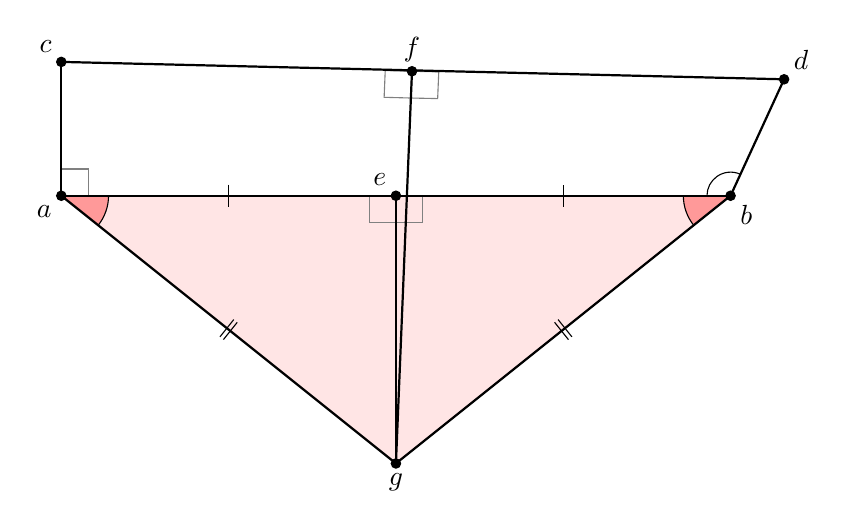
\begin{tikzpicture}[scale=1.7]
        \path (0,1) -- (5.5,-2);
        \coordinate (A) at  (0, 0);
        \coordinate (B) at  (5, 0);
        \coordinate (C) at  (0, 1);
        \coordinate (D) at  (5.4, .87);
        \coordinate (E) at  (2.5, 0);
        \coordinate (F) at  (2.62, .93);
        \coordinate (G) at  (2.5, -2);

        \tkzMarkRightAngle[size=.2,color=gray](C,A,B);
        \tkzMarkRightAngle[size=.2,color=gray](C,F,G);
        \tkzMarkRightAngle[size=.2,color=gray](D,F,G);
        
        \draw[fill=red!10] (A) -- (G) -- (E) -- cycle;
        \draw[fill=red!10] (B) -- (G) -- (E) -- cycle;

        \tkzMarkRightAngle[size=.2,color=gray](A,E,G);
        \tkzMarkRightAngle[size=.2,color=gray](B,E,G);
        
        \draw [-] pic [draw=black, angle radius=3mm] {angle = D--B--A};
        \draw [-] pic [draw=black, fill=red!40, angle radius=6mm] {angle = G--A--E};
        \draw [-] pic [draw=black, fill=red!40, angle radius=6mm] {angle = E--B--G};
        
        \tkzMarkRightAngle[size=.2,color=gray](C,A,B);
        
        \filldraw [] (A) circle (1pt) node[below left]{$a$};
        \filldraw [] (B) circle (1pt) node[below right]{$b$};
        \filldraw [] (C) circle (1pt) node[above left]{$c$};
        \filldraw [] (D) circle (1pt) node[above right]{$d$};
        \filldraw [] (E) circle (1pt) node[above left]{$e$};
        \filldraw [] (F) circle (1pt) node[above]{$f$};
        \filldraw [] (G) circle (1pt) node[below]{$g$};

        \tkzMarkSegment[mark=|](A, E)
        \tkzMarkSegment[mark=|](B, E)
        
        \tkzMarkSegment[mark=||](A, G)
        \tkzMarkSegment[mark=||](B, G)

        \draw[-, thick] (A) -- (B);
        \draw[-, thick] (A) -- (C);
        \draw[-, thick] (B) -- (D);
        \draw[-, thick] (C) -- (D);
        \draw[-, thick] (E) -- (G);
        \draw[-, thick] (F) -- (G);
        \draw[-, thick] (A) -- (G);
        \draw[-, thick] (B) -- (G);
    \end{tikzpicture}
\end{figure}

\vspace{.5cm}

Next, draw the line segments $\overline{ag}$ and $\overline{bg}$. These two segments form the legs of the isosceles triangle $\triangle abg$ (we know that $\triangle abg$ is isosceles since point $g$ lies on the perpendicular bisector of $\overline{ab}$). The fact that $\triangle abg$ is isosceles also tells us that angles $\angle eag$ and $\angle ebg$ (shown in pink) are congruent.

\newpage

% ----------------------------------------------------------------------------

\subsection{Step 5}

\vspace{.5cm}

\begin{figure}[ht]
    \centering
    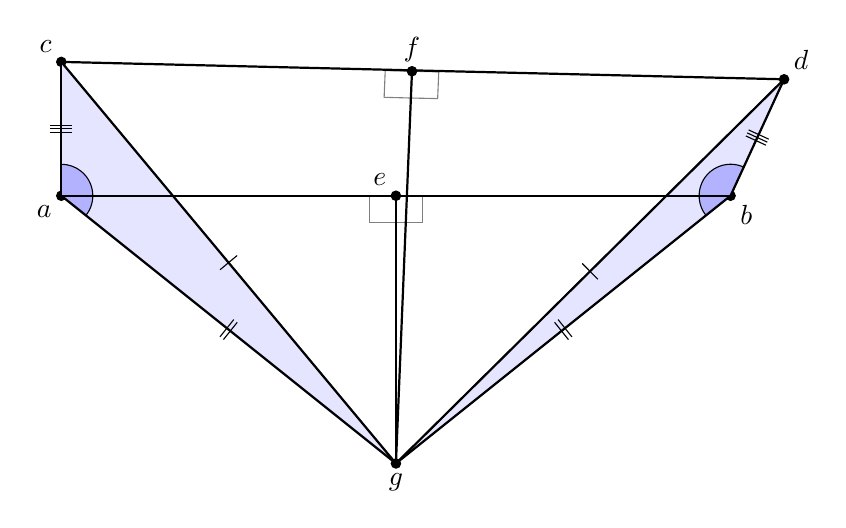
\begin{tikzpicture}[scale=1.7]
        \path (0,1) -- (5.5,-2);
        \coordinate (A) at  (0, 0);
        \coordinate (B) at  (5, 0);
        \coordinate (C) at  (0, 1);
        \coordinate (D) at  (5.4, .87);
        \coordinate (E) at  (2.5, 0);
        \coordinate (F) at  (2.62, .93);
        \coordinate (G) at  (2.5, -2);

        \tkzMarkRightAngle[size=.2,color=gray](C,F,G);
        \tkzMarkRightAngle[size=.2,color=gray](D,F,G);
        \tkzMarkRightAngle[size=.2,color=gray](A,E,G);
        \tkzMarkRightAngle[size=.2,color=gray](B,E,G);

        \filldraw [] (A) circle (1pt) node[below left]{$a$};
        \filldraw [] (B) circle (1pt) node[below right]{$b$};
        \filldraw [] (C) circle (1pt) node[above left]{$c$};
        \filldraw [] (D) circle (1pt) node[above right]{$d$};
        \filldraw [] (E) circle (1pt) node[above left]{$e$};
        \filldraw [] (F) circle (1pt) node[above]{$f$};
        \filldraw [] (G) circle (1pt) node[below]{$g$};

        \draw[fill=blue!10] (A) -- (G) -- (C) -- cycle;
        \draw[fill=blue!10] (B) -- (G) -- (D) -- cycle;

        \draw [-] pic [draw=black, fill=blue!30, angle radius=4mm] {angle = G--A--C};
        \draw [-] pic [draw=black, fill=blue!30, angle radius=4mm] {angle = D--B--G};

        \tkzMarkSegment[mark=|](C, G)
        \tkzMarkSegment[mark=|](D, G)

        \tkzMarkSegment[mark=||](A, G)
        \tkzMarkSegment[mark=||](B, G)


        \tkzMarkSegment[mark=|||](A, C)
        \tkzMarkSegment[mark=|||](B, D)

        \draw[-, thick] (A) -- (B);
        \draw[-, thick] (A) -- (C);
        \draw[-, thick] (B) -- (D);
        \draw[-, thick] (C) -- (D);
        \draw[-, thick] (E) -- (G);
        \draw[-, thick] (F) -- (G);
        \draw[-, thick] (A) -- (G);
        \draw[-, thick] (B) -- (G);
        \draw[-, thick] (C) -- (G);
        \draw[-, thick] (D) -- (G);
    \end{tikzpicture}
\end{figure}

\vspace{.5cm}

The last two line segments to draw are $\overline{cg}$ and $\overline{dg}$. As in the previous step, these segments are the legs of an isosceles triangle, in this case $\triangle cdg$, and therefore have equal length. This means that $\triangle acg \cong \triangle bdg$ by the side-side-side congruence rule, since $\overline{cg} \cong \overline{dg}$ (described above), $\overline{ag} \cong \overline{bg}$ (described in step 4), and $\overline{ac} \cong \overline{bd}$ (given in step 2).

\vspace{1cm}

Since triangles $\triangle acg$ and $\triangle bdg$ are congruent, we know that the corresponding angles in the triangles must be congruent. In particular, we know that angles $\angle cag$ and $\angle dbg$ (shown in purple) are congruent.

\newpage

% ----------------------------------------------------------------------------

\subsection{Step 6}

\vspace{.5cm}

\begin{figure}[ht]
    \centering
    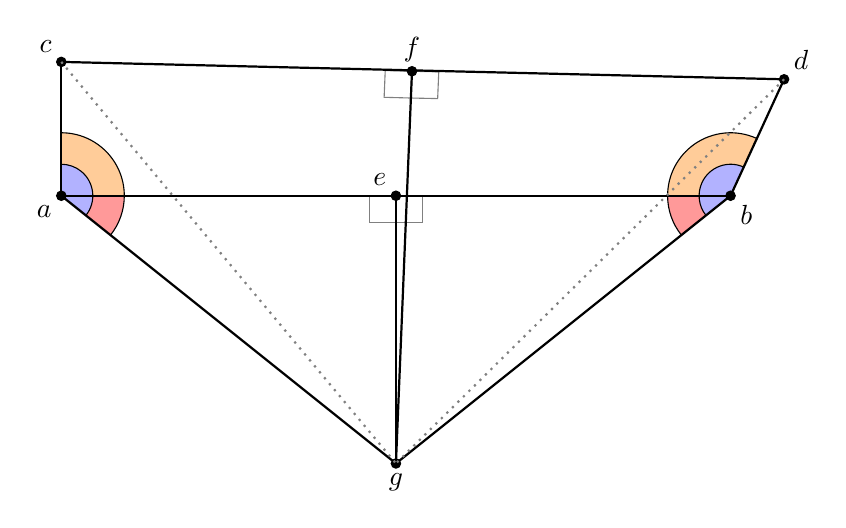
\begin{tikzpicture}[scale=1.7]
        \path (0,1) -- (5.5,-2);
        \coordinate (A) at  (0, 0);
        \coordinate (B) at  (5, 0);
        \coordinate (C) at  (0, 1);
        \coordinate (D) at  (5.4, .87);
        \coordinate (E) at  (2.5, 0);
        \coordinate (F) at  (2.62, .93);
        \coordinate (G) at  (2.5, -2);

        \tkzMarkRightAngle[size=.2,color=gray](C,A,B);
        \tkzMarkRightAngle[size=.2,color=gray](C,F,G);
        \tkzMarkRightAngle[size=.2,color=gray](D,F,G);

        \tkzMarkRightAngle[size=.2,color=gray](A,E,G);
        \tkzMarkRightAngle[size=.2,color=gray](B,E,G);

        \draw [-] pic [draw=black, fill=orange!40, angle radius=8mm] {angle = D--B--E};
        \draw [-] pic [draw=black, fill=orange!40, angle radius=8mm] {angle = E--A--C};
        \draw [-] pic [draw=black, fill=red!40, angle radius=8mm] {angle = G--A--E};
        \draw [-] pic [draw=black, fill=red!40, angle radius=8mm] {angle = E--B--G};
        \draw [-] pic [draw=black, fill=blue!30, angle radius=4mm] {angle = G--A--C};
        \draw [-] pic [draw=black, fill=blue!30, angle radius=4mm] {angle = D--B--G};

        \filldraw [] (A) circle (1pt) node[below left]{$a$};
        \filldraw [] (B) circle (1pt) node[below right]{$b$};
        \filldraw [] (C) circle (1pt) node[above left]{$c$};
        \filldraw [] (D) circle (1pt) node[above right]{$d$};
        \filldraw [] (E) circle (1pt) node[above left]{$e$};
        \filldraw [] (F) circle (1pt) node[above]{$f$};
        \filldraw [] (G) circle (1pt) node[below]{$g$};

        \draw[-, thick] (A) -- (B);
        \draw[-, thick] (A) -- (C);
        \draw[-, thick] (B) -- (D);
        \draw[-, thick] (C) -- (D);
        \draw[-, thick] (E) -- (G);
        \draw[-, thick] (F) -- (G);
        \draw[-, thick] (A) -- (G);
        \draw[-, thick] (B) -- (G);
        \draw[dotted, thick, gray] (C) -- (G);
        \draw[dotted, thick, gray] (D) -- (G);
    \end{tikzpicture}
\end{figure}

\vspace{.5cm}

From the previous two steps, we know that angles $\angle cag \cong \angle dbg$ (purple) and $\angle eag \cong \angle ebg$ (pink). Since $\angle cab = \angle cag - \angle eag$ and $\angle dba = \angle dbg - \angle ebg$, angles $\angle cab \cong \angle dba$ (orange). In other words, the purple angles are the sum of the pink and orange angles, which means that the orange angles are congruent, since the purple angles are congruent and the pink angles are congruent as well. 

\newpage

% ----------------------------------------------------------------------------

\subsection{Step 7}

\vspace{.5cm}

\begin{figure}[ht]
    \centering
    \begin{tikzpicture}[scale=1.7]
        \path (0,1) -- (5.5,0);
        \coordinate (A) at  (0, 0);
        \coordinate (B) at  (5, 0);
        \coordinate (C) at  (0, 1);
        \coordinate (D) at  (5.4, .87);
        
        \filldraw [] (A) circle (1pt) node[below left]{$a$};
        \filldraw [] (B) circle (1pt) node[below right]{$b$};
        \filldraw [] (C) circle (1pt) node[above left]{$c$};
        \filldraw [] (D) circle (1pt) node[above right]{$d$};

        \draw [-] pic [draw=black, fill=orange!40, angle radius=8mm] {angle = D--B--E};
        \draw [-] pic [draw=black, fill=orange!40, angle radius=8mm] {angle = E--A--C};
        
        \tkzMarkRightAngle[size=.2,color=gray](C,A,B);
        
        \draw [-] pic [draw=black, angle radius=3mm, above left] {angle = D--B--A};
        
        \draw[-, thick] (A) -- (B);
        \draw[-, thick] (A) -- (C);
        \draw[-, thick] (B) -- (D);
        \draw[-, thick] (C) -- (D);
    \end{tikzpicture}
\end{figure}

\vspace{.5cm}

We have shown that angles $\angle cab$ and $\angle dba$ are congruent. However, we know from step 1 that $\angle cab$ is a right angle, and that $\angle dba$ is obtuse (given in step 2). Thus, we have shown that an arbitrarily-chosen obtuse angle is congruent to a right angle. Given this fact, it is easy to show that all angles, acute or obtuse, are right angles\footnote{Left as an exercise for the reader}. \qed

\end{document}
